\documentclass{article}
\usepackage{geometry}
\geometry{a4paper, portrait, margin=1.5in}

\usepackage{hyperref}
\hypersetup{
    colorlinks=true,
    linkcolor=black,
    filecolor=magenta,
    urlcolor=blue,
}

\usepackage{graphicx}
\graphicspath{ {images/} }

\usepackage{tcolorbox}
\usepackage{textcomp}
\usepackage{gensymb}
\usepackage{indentfirst}

\title{RoboJackets Electrical Training Week 3 Worksheet}
\author{Alex Xu \\ Joe Spall}
\date{\today\\v1.2}
\begin{document}
\maketitle{}
\setcounter{tocdepth}{2}
\tableofcontents
\pagebreak

\section{Introduction}
In last week's training, we used Arduinos and some separate supporting electrical components to control motors. The Arduino board and the motor control circuitry exist independently from each other and is cumbersome if they're installed on the robot in their current state. A PCB that integrates all the components would be a lot more manageable when installed on a robot. That is the eventual goal of this training. \par
In this week, we will be \textbf{prototyping the PCB by replicating it on a breadboard} so we can verify that the circuit works. \textbf{\emph{Important steps that need to be taken are highlighted in bold-italic font.}}

\begin{figure}[!h]
    \center
    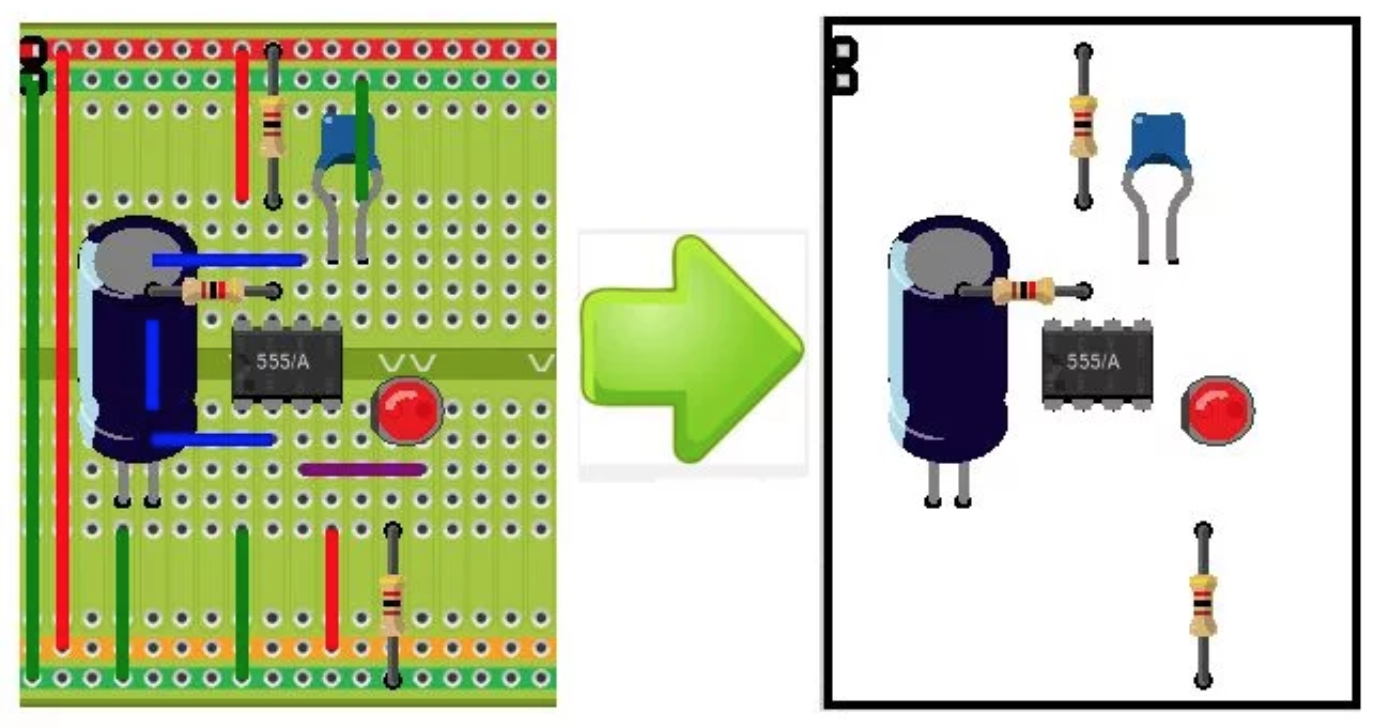
\includegraphics[width=0.6\textwidth,height=0.6\textheight,keepaspectratio]{breadboard_to_pcb}
    \caption {From breadboarding to a custom PCB}
\end{figure}

\section{Integrated Circuit Packages}
``The package is what encapsulates the integrated circuit die and splays it out into a device we can more easily connect to... There are many different types of packages, each of which has unique dimensions, mounting-types, and/or pin-counts.''  - SparkFun. \par
All packages can be divided in to two groups by their mounting types: through-hole or surface-mount (SMD or SMT). Through-hole packages are generally bigger and much easier to hand-solder. They're designed to be stuck through the holes on a board and soldered from the other side. Through-hole components are commonly used with a breadboard since they can be easily connected in the holes. SMD components are more commonly seen on PCBs and are much smaller at a cost of being more difficult to hand-solder. All of the packages to be used today will be through-hole components.

\begin{figure}[!h]
    \center
    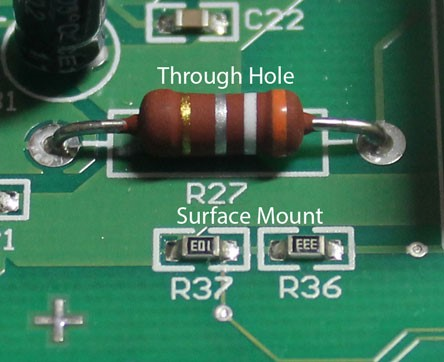
\includegraphics[width=0.4\textwidth,keepaspectratio]{throughvssmd}
    \caption {Through-hole components vs SMD}
    \label{img:through_vs_smd}
\end{figure}

\begin{figure}[!h]
    \center
    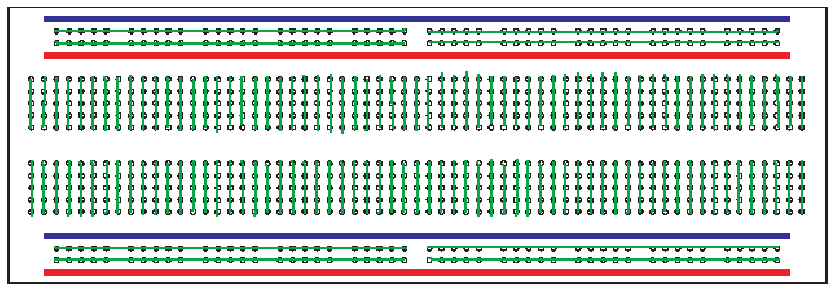
\includegraphics[width=0.8\textwidth,keepaspectratio]{Breadboard_Internal_Connections}
    \caption {Breadboard Internal Connections}
    \label{img:bread_connections}
\end{figure}

\section{Breadboarding}

\subsection{Placing the Important Chip}
\begin{table}[!h]
    \center
    \begin{tabular}{c|c|c}
        Name                    & Quantity & Package   \\
        \hline
        ATmega328               & 1        & DIP       \\
        DIP Socket              & 1        & DIP       \\
        Linear Regulator - 3.3V & 1        & TO-220-3  \\
        Capacitor - 10uF        & 1        & Radial    \\
        Capacitor - 0.1uF       & 1        & Radial    \\
        Capacitor - 22pF        & 2        & Radial    \\
        9V Battery Clip         & 1        & N/A       \\
        Crystal - 16MHz         & 1        & HC-49     
    \end{tabular}
    \caption{Component List for Breadboarding Lab}
    \label{table:componentList}
\end{table}

We will place our microcontroller (mcu), the \textbf{ATmega328}, first. \textbf{\emph{We place the ATmega328 component already in the DIP Socket (Ref Figure \ref{img:dip_socket}) into the breadboard}}. It is a Dual Inline Package (DIP), and the package needs to be placed as shown in Figure \ref{img:dip_breadboard}. 

\begin{figure}[!h]
    \center
    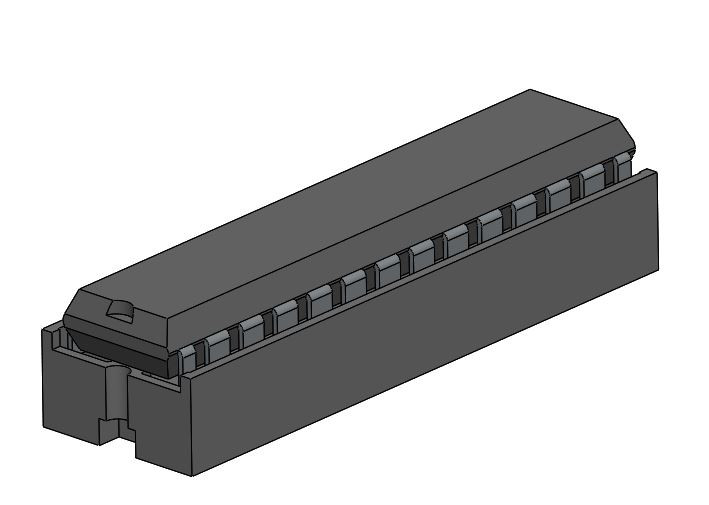
\includegraphics[width=0.4\textwidth,keepaspectratio]{dip_socket}
    \caption {CAD showing the ATmega328 in a DIP Socket}
    \label{img:dip_socket}
\end{figure}

\pagebreak

\begin{figure}[!h]
    \center
    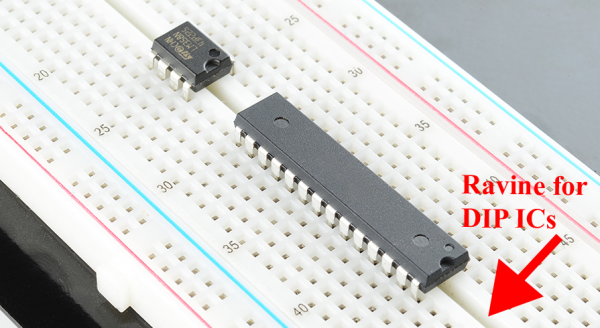
\includegraphics[width=0.4\textwidth,keepaspectratio]{dip_breadboard}
    \caption {Placing DIPs into breadboard}
    \label{img:dip_breadboard}
\end{figure}

\subsection{Adding Supporting Components}
The operation of our ATmega328 requires an external crystal. The operation of a crystal requires two supporting capacitors. \textbf{\emph{Insert the crystal and the two 22pF capacitors into the breadboard so it is equivalent to the schematic in Figure \ref{img:crystal}.}} GND means ground and refer to Figure \ref{img:bread_connections} for ground connections. Refer to the notch on one end of ATmega328 package and its datasheet for pin 9 and pin 10 location. \par

\begin{figure}[!h]
    \center
    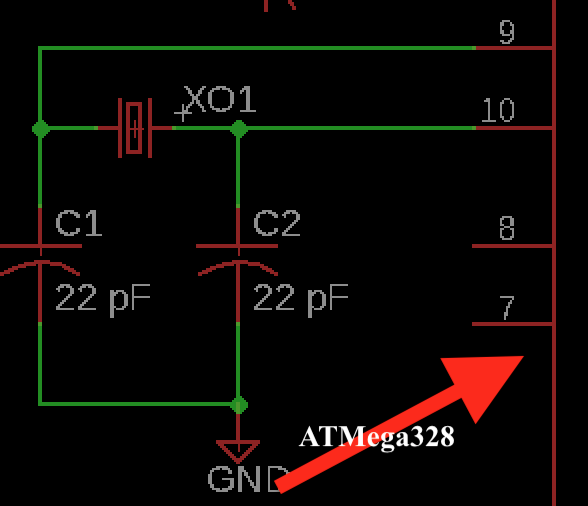
\includegraphics[width=0.4\textwidth,keepaspectratio]{crystal}
    \caption{The necessary crystal and capacitor connections}
    \label{img:crystal}
\end{figure}

The ATmega328 also requires a decoupling capacitor to operate. A decoupling capacitor smooths the power input into the Atmega. \textbf{\emph{Connect a 0.1uF capacitor between the power and ground pin of the ATmega.}}

\subsection{Adding Power Supply}
The next step would be the power supply. We want the ATmega to run at 3.3V to interface with a later project. However a 3.3V power supply is not very common. Therefore, we will use a 9V battery and use a linear regulator to transform the voltage to 3.3V. \par
Connect the blue line of battery clip to the ground connection on breadboard. Additionally, more decoupling capacitors are required for the power regulator. \emph{\textbf{Connect the linear regulator, the 9V battery clip, the 100nF capacitor, and 10uF capacitor as shown in Figure \ref{img:linear_regulator}}}. $V_{in}$ corresponds to the 9V from the battery clip and $V_{out}$ corresponds to 3.3V input for the ATmega. Connect the power rail on the breadboard to the $V_{out}$ pin and all of the GND pins together. 

\begin{figure}[!h]
    \center
    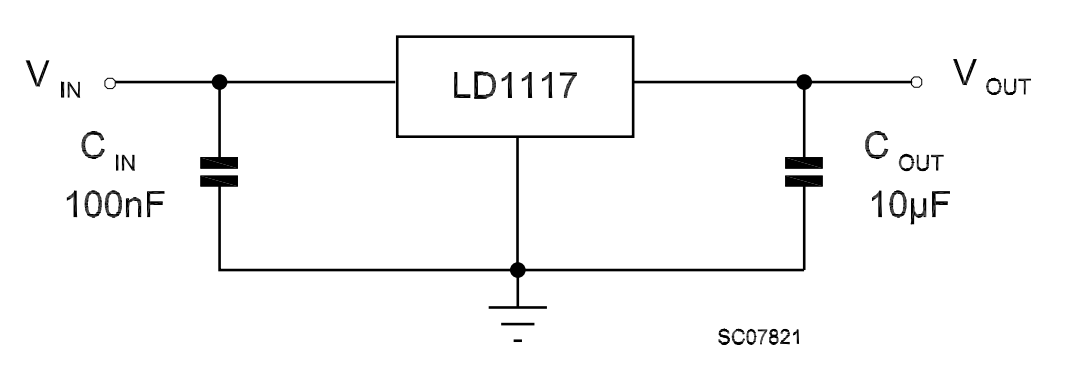
\includegraphics[width=0.8\textwidth,keepaspectratio]{linear_regulator}
    \caption{Power Circuit Schematics}
    \label{img:linear_regulator}
\end{figure}

\begin{tcolorbox} [title=Tips \& Tricks]
    \begin{itemize}
        \item The breadboard has multiple ground and power rails (red and blue). The ground rails need to be all connected if used and different ground rails \textbf{will} have to be connected via jumper wire.
        \item Power rails do not need to have the same voltage across the entire breadboard and not all voltage lines need to go on power rails. \textbf{Do not} connect power rails of different voltages together.
    \end{itemize}
\end{tcolorbox}

\subsection{Completing the Circuit}
\textbf{\emph{Connect all GND pins to the ground rail and all VCC pins to power rail.}} Use a multimeter to test the continuity between power and ground rail to make sure it's not shorted. Check the board connection with the Figure \ref{img:egBBL}.

\begin{figure}[h]
    \center
    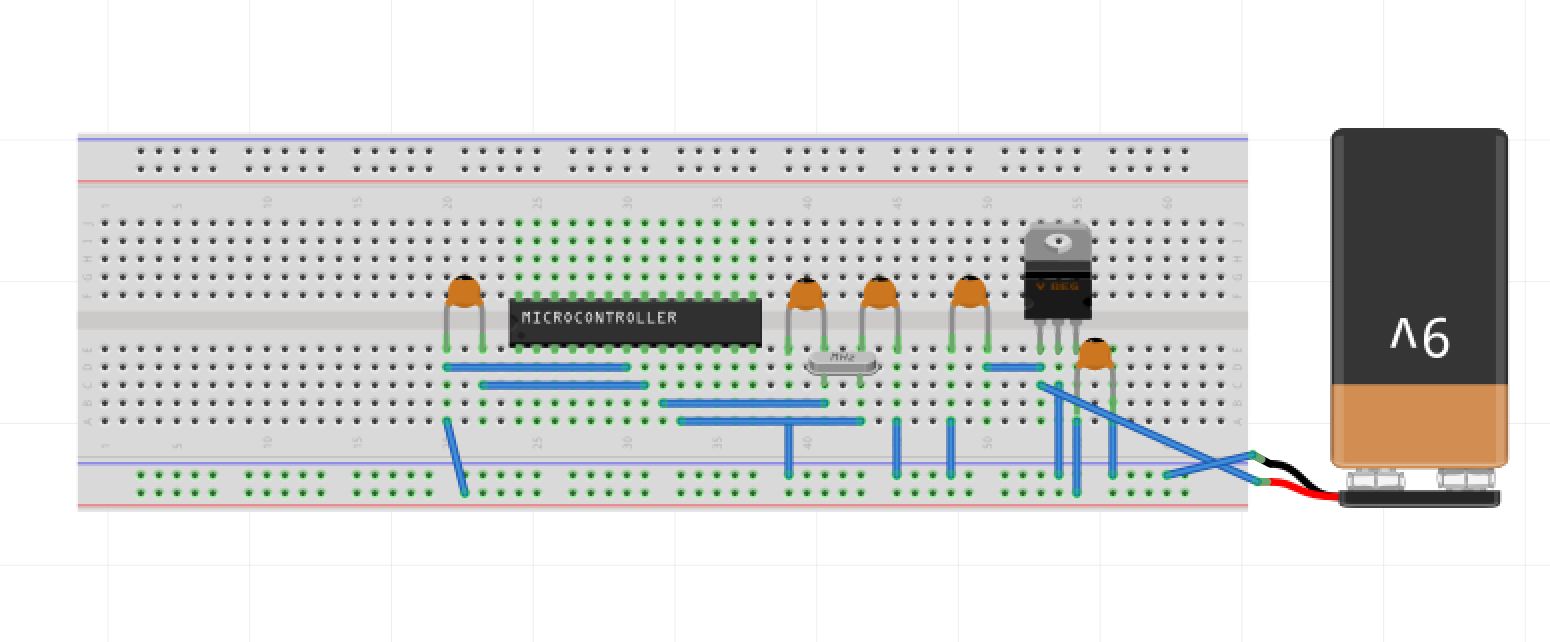
\includegraphics[width=\textwidth,keepaspectratio]{egBBL}
    \caption{Example Breadboard Layout}
    \label{img:egBBL}
\end{figure}

\section{Programming the Board}
Congratulations, you have just constructed a small-sized version of Arduino! Program the board to access its I/O pins and use it like an Arduino. 
\subsection{Burning the Bootloader}
On a microcontroller, the bootloader is the lower level program that loads your Arduino program for execution. If you have a new ATMega328, you'll need to burn the bootloader onto it. You can do this either using an Arduino board as an in-system program (ISP) or a Pocket AVR Programmer (recommended). If the microcontroller already has the bootloader on it (e.g. because you took it out of an Arduino board or ordered an already-bootloaded ATmega), you can skip this section. For training purposes, the micro-controller in your hand does not have a bootloader. \par
To burn the bootloader, follow these hardware setups: \par
\begin{enumerate}
    \item Add a 1k$\ohm$ resistor (Brown, Black, Red) between the RESETN pin and +5V on your ATmega328 circuit. 
    \item Connect MOSI, MISO, SCK, Reset, power and ground to the Pocket AVR Programmer. Pocket AVR Programmer cable 2x3 connector pinout is specified in Fig \ref{img:avr_pinout_fig}. ATMega328 pinout specified in Fig \ref{img:atmega_pinout_fig}.
\end{enumerate}

\begin{figure}[h]
    \center
    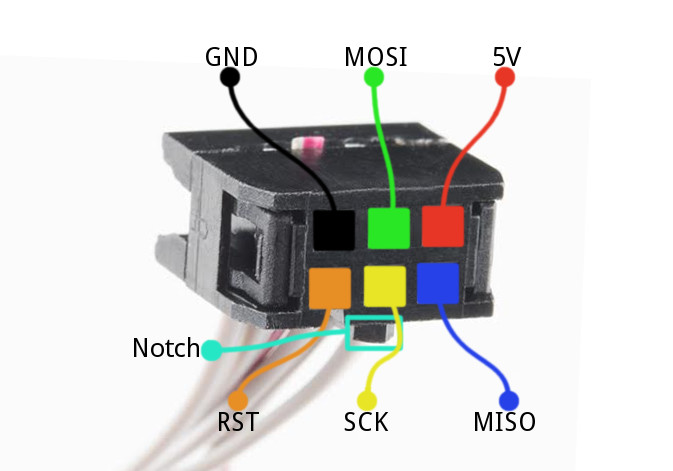
\includegraphics[width=0.5\textwidth,keepaspectratio]{avr_pinout}
    \caption{Pocket AVR Programmer programming cable pinout}
    \label{img:avr_pinout_fig}
\end{figure}

\begin{figure}[h]
    \center
    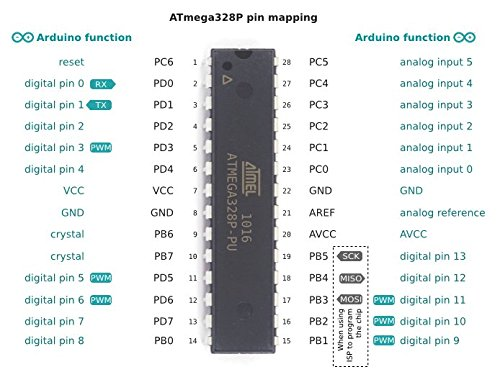
\includegraphics[width=0.7\textwidth,keepaspectratio]{atmega_pinout}
    \caption{ATMega328 DIP package pinout}
    \label{img:atmega_pinout_fig}
\end{figure}

We additionally recommend using this custom library for uploading the bootloader:
\begin{enumerate}
    \item In Arduino IDE, Open the File $>$ Preferences menu item.
    \item Enter the following URL in Additional Boards Manager URLs: \url{https://mcudude.github.io/MiniCore/package_MCUdude_MiniCore_index.json}.
    \item Open the Tools $>$ Board $>$ Boards Manager... menu item.
    \item Search for MiniCore and click on it, click Install when the button appears.
\end{enumerate}
Once you have the library installed, close the Boards Manager and follow these steps:
\begin{enumerate}
    \item Select "ATmega328" from the Tools $>$ Board menu.
    \item Select "USBtinyISP" from Tools $>$ Programmer
    \item Run Tools $>$ Burn Bootloader
\end{enumerate}

You should only need to burn the bootloader once. After you've done so, you can remove the jumper wires connected to AVR programmer. There are also ways to burn the bootloader using another Arduino that already has bootloader burnt. For more information on that method, visit Arduino.cc. 

\subsection{Uploading Using an Arduino Board}
Notice: The following subsection is based on Arduino.cc ``From Arduino to a Microcontroller on a Breadboard" tutorial. \par
Once your ATmega328p has the Arduino bootloader on it, you can upload programs to it using the USB-to-serial convertor (FTDI chip) on an Arduino board. \par In order to do this, remove the microcontroller from the Arduino board so the FTDI chip can talk to the microcontroller on the breadboard instead. The diagram at Figure \ref{img:ArduinoUSBSerial} shows how to connect the RX and TX lines from the Arduino board to the ATmega on the breadboard. To program the microcontroller, select ``Arduino/Genuino Uno" from the the Tools $>$ Board menu. Then upload as usual.

\begin{figure}[!h]
    \center
    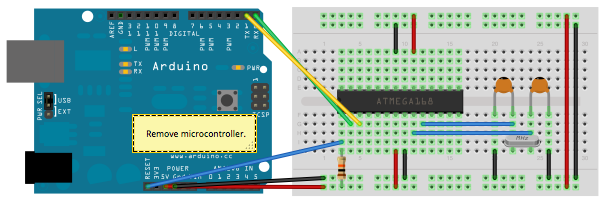
\includegraphics[width=0.6\textwidth,keepaspectratio]{ArduinoUSBSerial}
    \caption{Programming an ATmega from an Arduino}
    \label{img:ArduinoUSBSerial}
\end{figure}

You can also upload your program using the Pocket AVR Programmer. You will need to use "Upload Using Programmer" instead of ``Upload".

\subsection{Upload Your Program!}
Now verify everything works by replicating one of the circuits and programs you had from earlier labs, such as blinky.

\end{document}